\documentclass{scrartcl}
\usepackage[utf8]{inputenc}
\usepackage[T1]{fontenc}
\usepackage[ngerman]{babel}
\usepackage{amssymb}
\usepackage{amsmath}
\usepackage{graphicx}
\usepackage{framed}
\usepackage{xcolor}
\colorlet{shadecolor}{gray!25}
\setlength{\parindent}{0pt}

\newcommand{\abs}[1]{\left\lvert#1\right\rvert}

\begin{document}
% ----------------------------------------------------------------------
\title{Approximation von Ableitungen\\mittels finiter Differenzen}
\author{Marisa Breßler und Anne Jeschke}
\date{08.11.2019}
\maketitle
% ----------------------------------------------------------------------------
% Inhaltsverzeichnis:
\tableofcontents
% ----------------------------------------------------------------------------
% Gliederung und Text:
\pagebreak \section{Einleitung}
\label{sec:einleitung}
Im Gegensatz zur Analysis bietet die Numerik praktikable Näherungen an Real- bzw. Idealbilder. Die Güte dieser Näherung ist im Minimum abschätzbar, bleibt also unterhalb einer beweisbaren Toleranzgrenze. \\
Ableitungen von Funktionen spielen in der Praxis eine große Rolle. So dienen die erste und die zweite Ableitung in der Physik zum Beispiel der Untersuchung von Bewegungsabläufen, wo die Geschwindigkeit und Beschleunigung definiert werden als erste und zweite Ableitung des Weges nach der Zeit. Änderungsprozesse müssen in ganz unterschiedlichen Kontexten erfasst und/oder vorausgesagt werden. Dabei ist es in einer Vielzahl von Praxisbeispielen notwendig, Ableitungen zu approximieren. Unter Umständen ist eine Funktion zwar durch Formeln bekannt, doch das exakte Differenzieren gestaltet sich als aufwändig oder das Ermitteln von Funktionswerten als schwierig, weil die Ableitungsfunktion von sehr komplexer Natur ist. Das näherungsweise Differenzieren hat eines ihrer Hauptanwendungsgebiete bei der Verarbeitung von Messwerten. Hier ist die Funktion im Allgemeinen nicht explizit bekannt, das heißt sie liegt nicht in analytischer Form, sondern nur in Form von diskreten Punkten vor. Aufgrund der gegebenen lückenhaften Informationen ist die Ableitung mit analytischen Methoden der Differentialrechnung nicht exakt bestimmbar. An dieser Stelle werden numerische Verfahren verwendet, um die Ableitungen beziehungsweise die Werte der Ableitungen an bestimmten Stellen mit einer gewissen Genauigkeit näherungsweise zu ermitteln. \\
\linebreak
\textit{Numerik beantwortet die Frage: Was bleibt vom Ableitungsbegriff übrig, wenn alle Rechnungen in endlich vielen Schritten und mit endlich vielen Zahlen in endliche vielen Ziffern abgehandelt werden müssen?} (Schneebeli, S. 4)\\
\linebreak
Numerisches Differenzieren ist zum Beispiel mit den sogenannten finiten Differenzen möglich. Diese stellen eine überschaubares Verfahren zum Approximieren von Ableitungen zur Verfügung. Auf welche Weise und wie gut, das heißt mit welcher Genauigkeit, das funktioniert, soll im Folgenden erläutert werden. \\

\pagebreak \section{Theorie}
\label{sec:theorie}
Die Formeln der finiten Differenzen, auch Differenzenformeln genannt, lassen sich auf verschiedene Weisen herleiten. Im Folgenden wollen wir zwei Ansätze vorstellen: Zum einen ist das ein geometrischer Ansatz, der die Definition der Ableitung über den Differentialquotienten nutzt, d.h. den Anstieg der Tangente an der zu untersuchenden Funktion an der zu betrachtenden Stelle. Zum anderen ist es ein Ansatz, der sich die Eigenschaften der Taylorentwicklung zunutze macht.

\subsection{Vom Differenzen- zum Differentialquotienten und umgekehrt}
\label{ssec:herleitung1}
Der Ausgangspunkt unserer geometrischen Herleitung der Differenzenformeln bildet die Definition der Ableitung:
\begin{shaded}
Eine Funktion $f:D \rightarrow \mathbb{R}$ (mit $D\subset \mathbb{R}$) heißt differenzierbar an der Stelle $x_0 \in D$, falls folgender Grenzwert existiert (mit $(x_0+h) \in D$): \[f'(x_0) = \lim _{x\to x_0} {\frac {f(x)-f(x_0)}{x-x_0}} = \lim _{h\to 0} {\frac {f(x_0+h)-f(x_0)}{h}}\] Dieser Grenzwert heißt \textit{Differentialquotient} / \textit{Ableitung} von $f$ nach $x$ an der Stelle $x_0$.
\end{shaded}
Der Differentialquotient geht zurück auf die Sekantensteigung. Ist die Ableitung einer Funktion $f$ an einer Stelle $x_0$ gesucht, wird wie eingangs erwähnt nach der Steigung der Tangente am Graphen von $f$ im Punkt $(x_0 \mid f(x_0))$ gefragt. Die Tangentensteigung kann näherungsweise mit der Sekantensteigung durch die Punkte $(x_0 \mid f(x_0))$ und $(x_0 + \Delta x \mid f(x_0 + \Delta x))$ bestimmt werden. Die Formel der Sekantensteigung durch die Punkte $(x_0 \mid f(x_0))$ und $(x_0 + \Delta x \mid f(x_0 + \Delta x))$ ist der folgende Differenzenquotient: \[\frac {f(x_0 + \Delta x)-f(\Delta x)}{(x_0 + \Delta x) - x_0} = \frac {f(x_0 + \Delta x)-f(\Delta x)}{\Delta x}\]
Setzt man $\Delta x =: h$ und lässt $h$ gegen $0$ laufen, erhält man die Formel für den Differentialquotienten, sprich für die Ableitung von $f$ an der Stelle $x_0$. Allerdings kann der Computer den Grenzübergang der sogenannten \textit{Schrittweite} $h$ gegen $0$ nicht leisten. Deswegen wählt man den Differenzenquotienten als Näherung der Ableitung. Werden Rundungsfehler vernachlässigt, die ein Computer immer aufgrund seiner begrenzten Genauigkeit in der Zahldarstellung verursacht, geht der numerische Wert des Differenzenquotienten gegen den exakten Wert der Ableitung. Aber auch in der Praxis gilt die Faustregel: Je kleiner die Schrittweite $h$ gewählt wird, desto genauer ist die numerische Näherung. \\
Der Differenzenquotient misst also die mittlere spezifische Änderung von $f$ zwischen zwei Stellen. Man unterscheidet zwischen dem \textit{rechtsseitigem Differenzenquotienten}, bei dem die Steigung der Sekante durch $x$ und $x+h$ berechnet wird, und dem \textit{linksseitigen Differenzenquotienten}, bei dem wiederum die Steigung der Sekante durch $x-h$ und $x$ berechnet wird. Allerdings ist die Nutzung des links- oder des rechtsseitigen Differenzenquotienten, einer \textit{finiten Differenz erster Ordnung} suboptimal, vor allem für einseitig gekrümmte Funktionsgraphen, bei denen oft eine sehr hohe Abweichung zwischen Sekanten- und Tangentensteigung zu beobachten ist. Deshalb kann es unter Umständen sinnvoll sein, diesen Fehler durch Mittelung zu verkleinern und das arithmetische Mittel der beiden einseitigen (asymmetrischen) Differenzenquotienten zu betrachten, das heißt die Sekantensteigung zwischen $x-h$ und $x+h$. Dies bezeichnet man als \textit{zentralen} oder auch \textit{symmetrischen Differenzenquotienten erster Ordnung}. Durch erneutes Anwenden der symmetrischen Differenzenformel für die erste Ableitung lässt sich eine symmetrische Differenzenformel zur Approximation der zweiten Ableitung gewinnen: der \textit{symmetrische Differenzenquotient zweiter Ordnung} bzw. die \textit{zweite finite Differenz}. Für höhere Ableitungen geht man analog vor. 
\begin{shaded}
\begin{center}
 rechtsseitiger Differenzenquotient / finite Differenz erster Ordnung:
 \end{center} \[ \frac {f(x+h) - f(x)}{h} \] 
\begin{center}
 linkssseitiger Differenzenquotient / finite Differenz erster Ordnung:
 \end{center} \[ \frac {f(x) - f(x-h)}{h} \] 
\begin{center}
 symmetrischer Differenzenquotient erster Ordnung:
 \end{center} \[ \frac {f(x+h) - f(x)}{h} \] 
\begin{center}
 symmetrischer Differenzenquotient zweiter Ordnung / zweite finite Differenz:
 \end{center} \[ \frac{f(x+h)-2f(x)+f(x-h)}{h^2} \] 
\end{shaded}

\subsection{Approximieren von Ableitungen via Taylorentwicklung}
\label{ssec:herleitung2}
Auch mit Hilfe der Taylorentwicklung einer Funktion lassen sich Formeln zur Approximation der Ableitungen einer Funktion herleiten. Betrachtet man auf einem Intervall $[a,b] \in \mathbb{R}$ eine reelle Funktion $f \in C^\infty([a,b])$, so kann man die Ableitung an einer Stelle $x \in (a,b)$ annähernd bestimmen, indem man zusätzlich eine in der Nähe liegende Stelle $(x+h) \in [a,b]$ mit $0<h \in \mathbb{R}$ betrachtet und den Funktionswert von $f$ an dieser Stelle $x+h$ mit Hilfe der Taylorentwicklung approximiert:
\[f(x+h) = \sum_{n=0}^{\infty}\frac{f^{(n)}(x)}{n!}h^n = f(x)+f'(x)h+\frac{f''(x)}{2}h^2+...\]
Wenn man diese Formel entsprechend äquivalent umformt, erhält man die Formel für die \textbf{\textit{erste finite Differenz}} von $f$ an der Stelle $x$:
\begin{shaded}
\[(D_h^{(1)}f)(x) = \frac{f(x+h)-f(x)}{h} = f'(x)+\sum_{n=2}^{\infty}\frac{f^{(n)}(x)}{n!}h^{n-1}=f'(x)+\mathcal{O}(h)\;\]
\end{shaded}
Die erste finite Differenz von $f$ an der Stelle $x$ entspricht also bis auf einen linearen Fehlerterm der ersten Ableitung von $f$ an der Stelle $x$. \\
Auch die zweite Ableitung von $f$ an der Stelle $x$ können wir auf ähnliche Weise mittels Funktionswerten von $f$ approximieren. Dazu benötigen wir zusätzlich die Taylorentwicklung von $f$ an der Stelle $(x-h) \in [a,b]$, das ebenfalls in der Nähe von $x$ liegt:
\[f(x-h) = \sum_{n=0}^{\infty}\frac{f^{(n)}(x)}{n!}(-h)^n = f(x)-f'(x)h+\frac{f''(x)}{2}h^2+...\]
Durch Aufsummieren der beiden Formel für die Taylorentwicklung um $x+h$ und $x-h$ und äquivalentes Umformen erhält man die Formel für die \textbf{\textit{zweite finite Differenz}} von $f$ an der Stelle $x$:
\begin{shaded}
\[(D_h^{(2)}f)(x) = \frac{f(x+h)-2f(x)+f(x-h)}{h^2} = f''(x)+\frac{f^{(4)}(x)h^2}{3\cdot4}+...=f''(x)+\mathcal{O}(h^2)\;\]
\end{shaded}
Diese entspricht wiederum der zweiten Ableitung von $f$ an der Stelle $x$ bis auf einen quadratischen Fehlerterm.

\subsection{Fehler und Schrittweite}
\label{ssec:schrittweite}
Die Fehler numerischer Berechnungen gegenüber exakter analytischer setzen sich ganz allgemein zusammen aus \textit{Verfahrensfehlern} und \textit{Rundungsfehlern}. Der Verfahrensfehler gibt den Unterschied zwischen dem exakten Wert der Ableitung an der Stelle $x$ und dem exakten Wert des Differenzenquotienten an der Stelle $x$ an. Rundungsfehler sind hingegen darauf zurückzuführen, dass der Computer aufgrund eines begrenzten Speichers Zahlen nur mit endlicher Genauigkeit darstellen und verarbeiten kann. Er verfügt lediglich über einen endlichen Vorrat an sogenannten Maschinenzahlen. Gibt der Benutzer eine Zahl in den Computer ein, die keine Maschinenzahl ist, wird sie zur nächstgelegenen Maschinenzahl gerundet. So kommt es insbesondere in dem Bereich der reellen Zahlen bereits bei der Übergabe von Zahlen an den Computer zu Rundungsfehlern. Aber auch nach jeder Operation rundet die Maschine und produziert damit weitere Rundungsfehler. Die Verstärkung der Rundungsfehler wird als \textit{Fehlerfortpflanzung} bezeichnet. Wie problematisch diese Fehler sind, ist von den Zahlen, der Art und der Reihenfolge der ausgeführten Operationen abhängig. In der Computerarithmetik sind Addition und Multiplikation zwar kommutativ, jedoch gelten Assoziativ- und Distributivgesetze im Allgemeinen nicht. Demnach können analytisch äquivalente Ausdrücke auf dem Computer zu erheblich unterschiedlichen Ergebnissen führen. \\
Ein heikler Punkt bei der Approximation der Ableitungen mit Differenzenquotienten ist die Wahl der Schrittweite $h$.
Ein zu großes $h$ führt zu Verfahrensfehlern, ein zu kleines $h$ birgt die Gefahr der \textit{Auslöschung}.
Die Subtraktion fast gleich großer Zahlen (die wir bei unseren Differenzenformeln für die erste und zweite Ableitung im Zählerterm finden) kann dazu führen, dass die Differenz zwischen den beiden Zahlen für den Computer nicht mehr erfassbar ist und signifikante Stellen \textit{ausgelöscht} werden.
So wird der Approximationsfehler beim Vermindern der Schrittweite zunächst kleiner, da die Funktionalität des Verfahrens und damit die Genauigkeit der Näherung steigt.
Allerdings macht sich im Laufe der Zeit die eben benannte Grenze bemerkbar. Bei sehr kleinen Schrittweiten muss mit Auslöschung gerechnet werden und damit wieder mit einer sinkenden Genauigkeit.
Ist das Ziel, möglichst genau zu approximieren, sollte man dieses "`optimale"' $h$ ausfindig machen.
Unter Umständen genügen aber bereits gröbere Näherungen und andere Faktoren spielen eine wichtigere Rolle (siehe hierzu unsere Zusammenfassung). \\

\pagebreak \section{Experimente und Beobachtungen}
\label{sec:experimente}

Wir betrachten zunächst die Funktion $g_1:[\pi, 3\pi] \rightarrow \mathbb{R}$ mit $g_1(x) = sin(x)/x$. Mit Hilfe eines in Python verfassten Programmes lassen wir folgende Graphen zeichnen (Funktionenplot): den von $g_1$, den der exakten ersten und zweiten Ableitung $g_1'$ und $g_1''$, die wir nach den analytischen Methoden der Differentialrechnung ermittelt haben, sowie den der ersten finiten Differenz $D_h^{(1)}g$ und den der zweiten $D_h^{(2)}g$. Für die Auswertung der genannten Funktionen durch den Computer unterteilen wir den Definitionsbereich $[\pi, 3\pi]$ in $p = 1000$ äquidistante Intervalle; nur an den Intervallgrenzen soll ausgewertet werden. Nun wollen wir die exakte und die approximierte erste und zweite Ableitung von $g_1$ für die Schrittweiten $h = \pi/3$, $h = \pi/4$, $h = \pi/5$ und $h = \pi/10$ graphisch vergleichen. \\
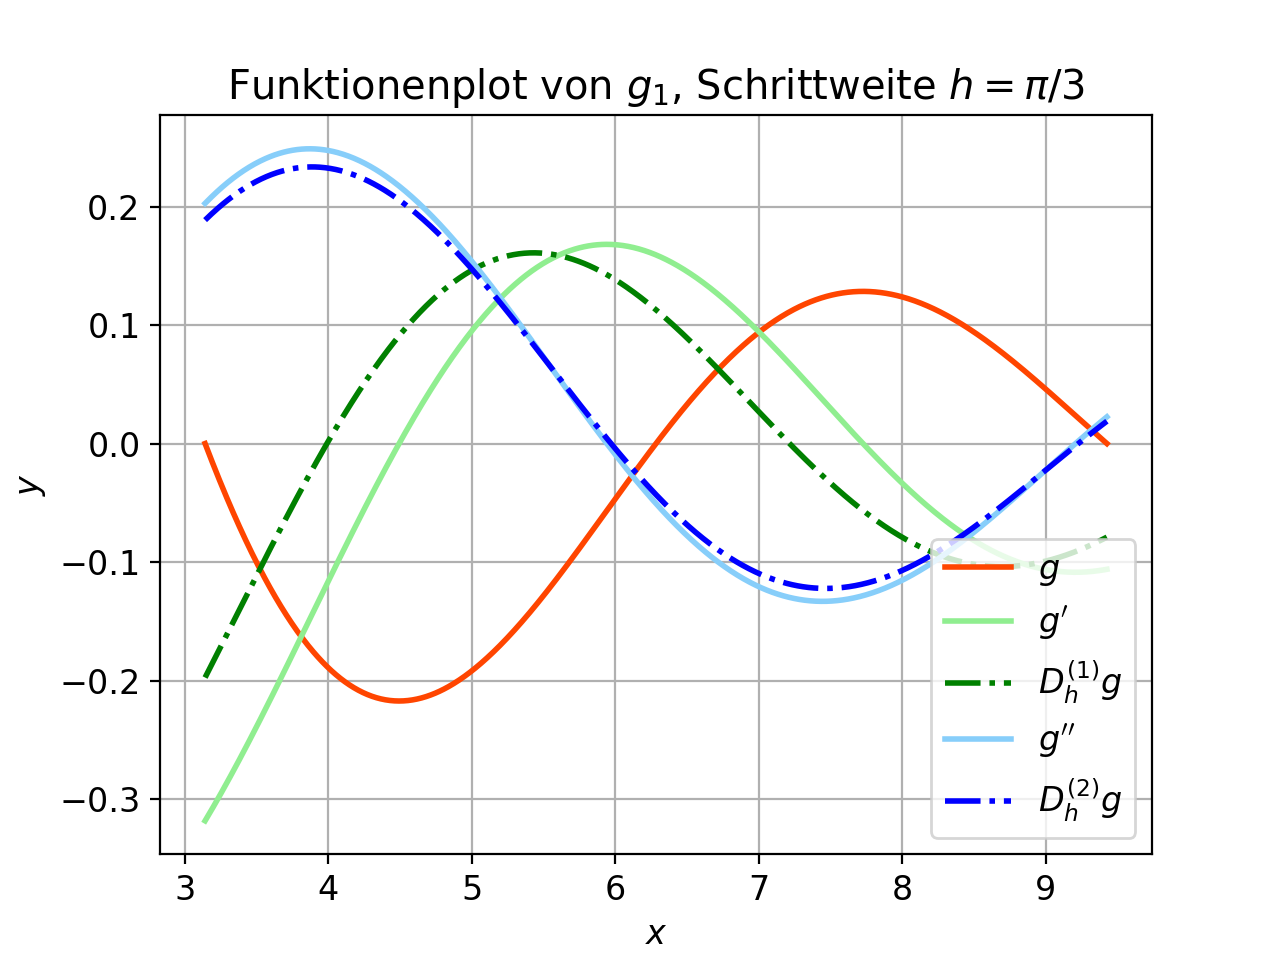
\includegraphics[width=0.5\textwidth]{Grafiken/Funktionenplot_Pi_Drittel} 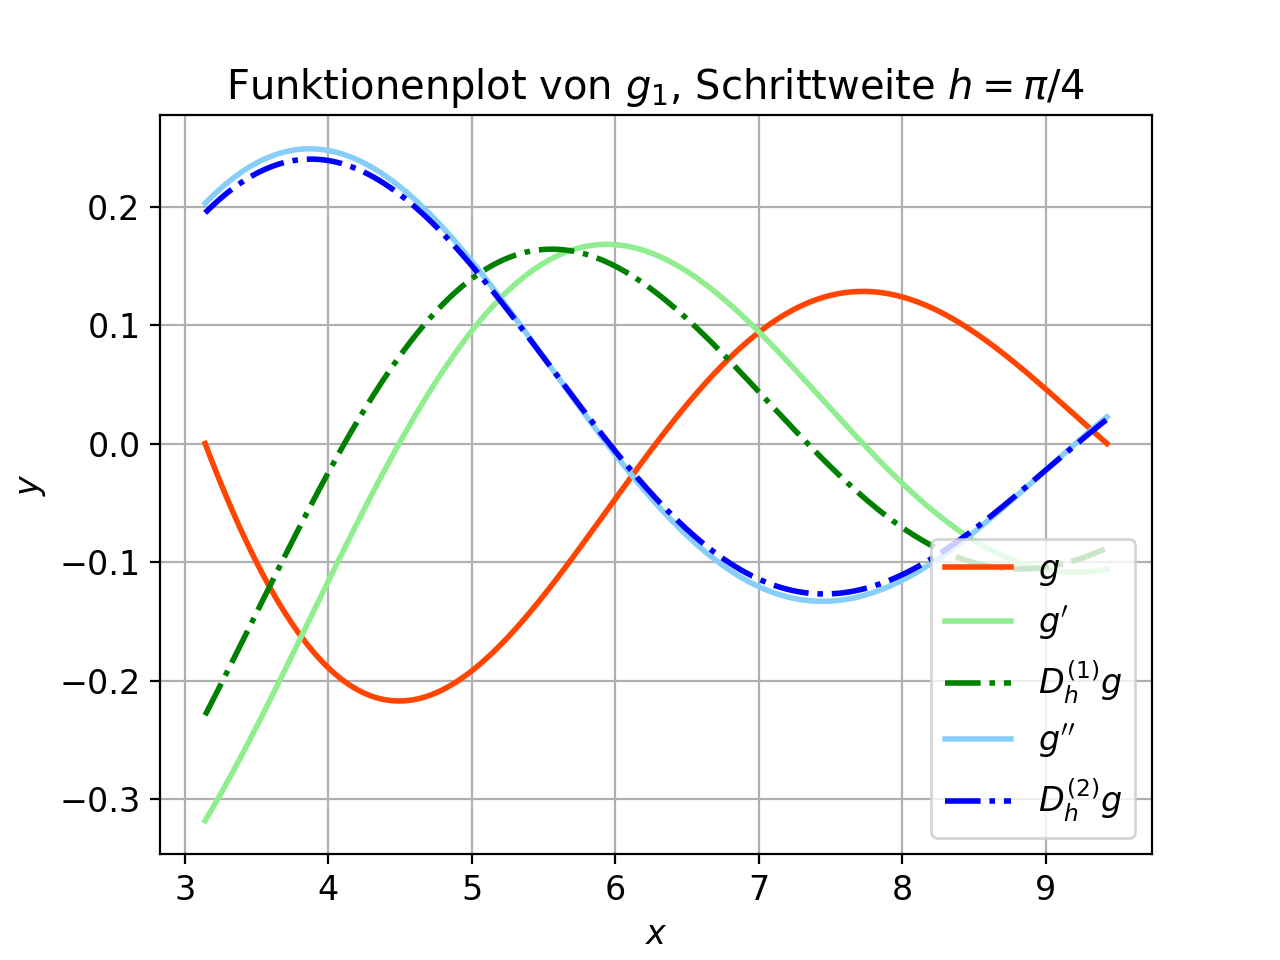
\includegraphics[width=0.5\textwidth]{Grafiken/Funktionenplot_Pi_Viertel}\\
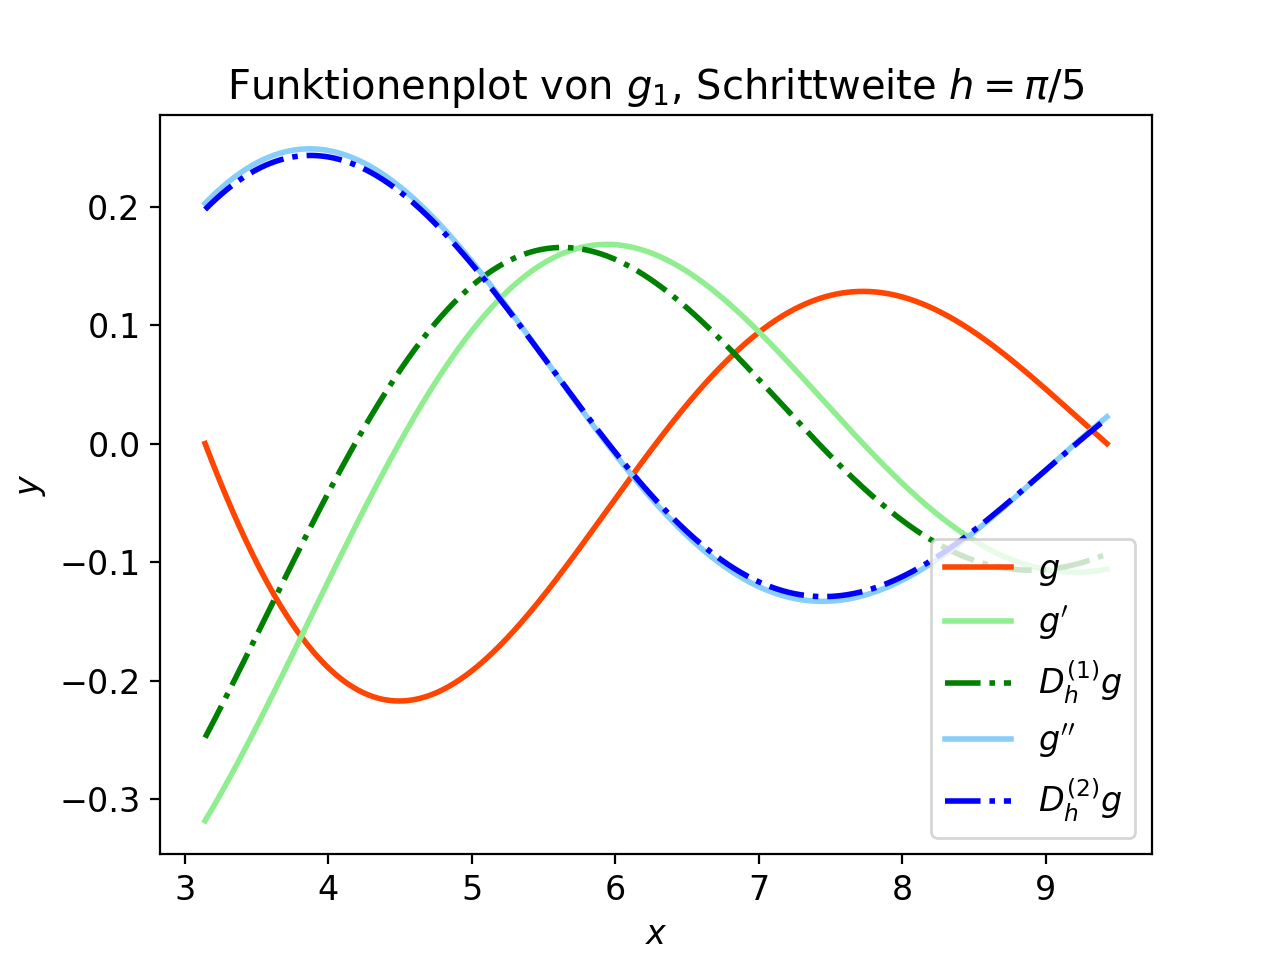
\includegraphics[width=0.5\textwidth]{Grafiken/Funktionenplot_Pi_Funftel} 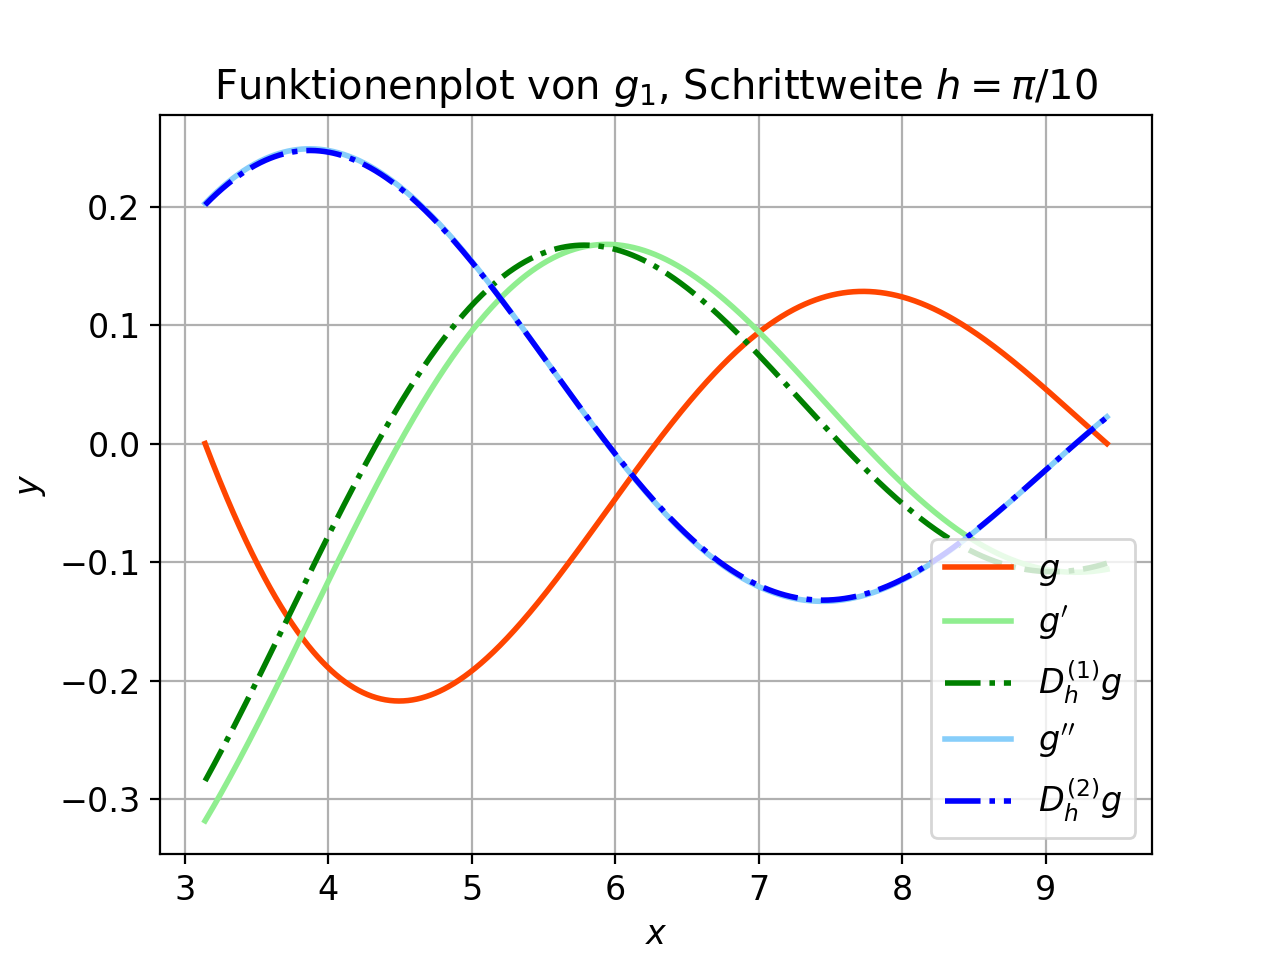
\includegraphics[width=0.5\textwidth]{Grafiken/Funktionenplot_Pi_Zehntel} \\
Allgemein ist folgender Zusammenhang erkennbar: je kleiner die Schrittweite, desto besser die Approximation. Darüber hinaus fällt auf, dass für alle $h$ die Näherung der jeweiligen Ableitung mittels zweiter finiter Differenz besser als die mittels erster finiter Differenz. Bereits mit der gröbsten Schrittweite $h = \pi/3$ ist die Approximation der zweiten Ableitung gut. Eine vergleichbar gute Approximation der ersten Ableitung erhalten wir erst mit der feinsten Schrittweite $h = \pi/10$. Bei dieser Schrittweite liegt der Graph der approximierten zweiten Ableitung bereits so gut wie auf dem Graphen der exakten. \\
 \\
Um das Konvergenzverhalten der Finite-Differenzen-Verfahren erster und zweiter Ordnung graphisch zu untersuchen, lassen wir bei gleich bleibenden Parametern ($g_1$, $[\pi, 3\pi]$, $p = 1000$) die maximalen absoluten Fehler in Abhängigkeit von der Schrittweite $h$ in einem Fehlerplot ausgeben, wobei die Referenzwerte die exakten Ableitungen zur Verfügung stellen. Dabei bezeichne $e_g^{(1)}$ den Fehler bei der ersten finiten Differenz und $e_g^{(2)}$ den Fehler bei der zweitem finiten Differenz. Wir betrachten die Approximationsfehler in der Maximumnorm mit der Formel (wobei die $x_i$'s die Intervallgrenzen unserer äquidistanten Unterteilen sind):
\[e_f^{(k)}(h):=\max_{i=0,..,p}\abs{f^{(k)}(x_i)-(D_h^{(k)}f)(x_i)} , k \in \lbrace1, 2\rbrace\]
Folgende Werte für $h$ sollen ausgewertet werden: $10^{-10}$, $5 \cdot 10^{-10}$, $10^{-9}$, $5 \cdot 10^{-9}$, ... , $10^{-1}$, $5 \cdot 10^{-1}$, $1$, $5$, $10$.
Um in der Grafik erkennen zu können, mit welcher Geschwindigkeit sich die maximalen Approximationsfehler ändern, lassen wir zudem die Graphen von $h \mapsto h$, $h \mapsto h^{2}$ und $h \mapsto h^{3}$ zeichnen und wählen die Darstellung in einem doppeltlogarithmischen Plot. 
\begin{figure}[h!]
	\centering
	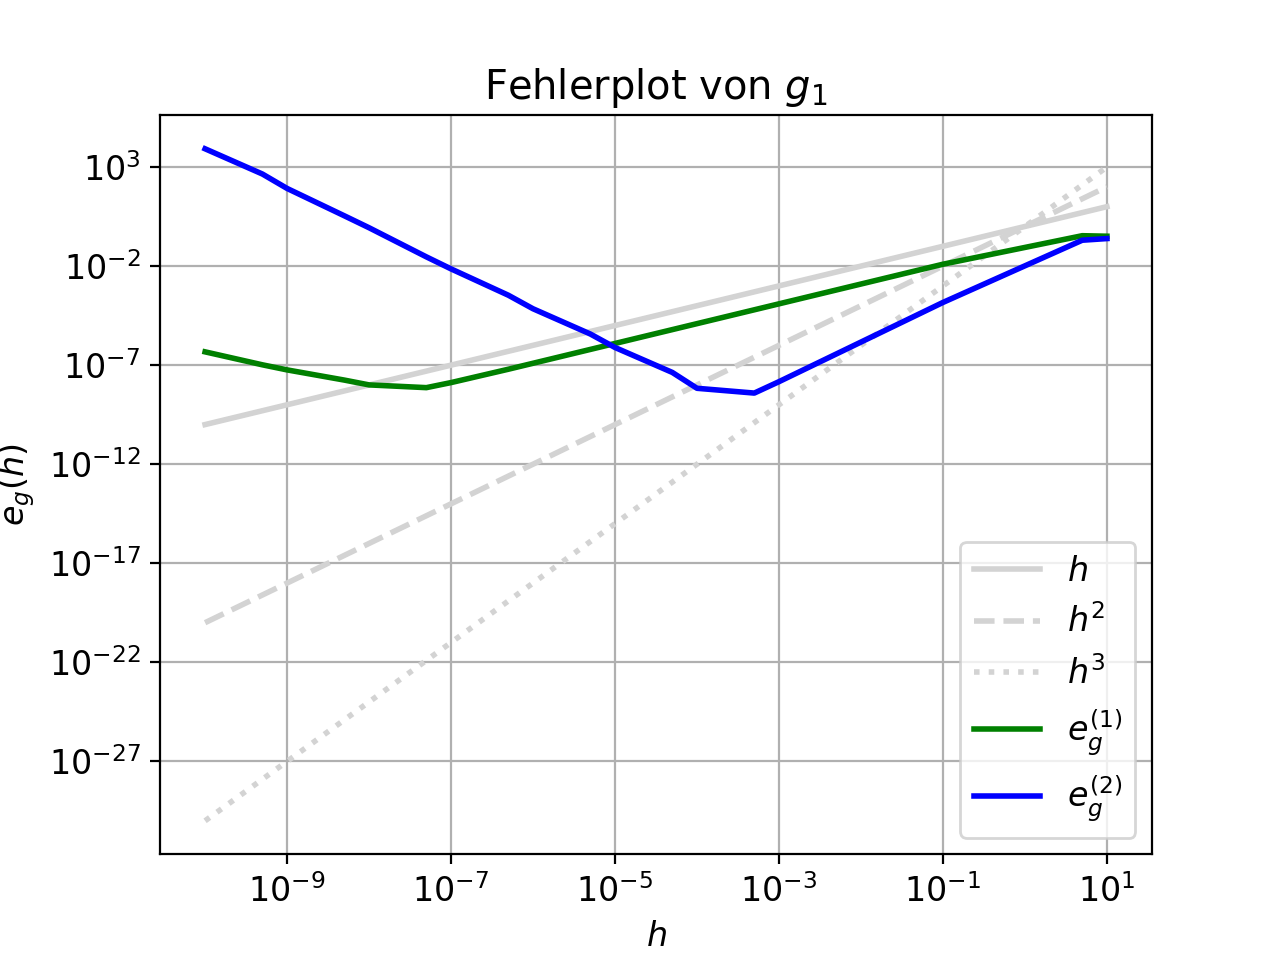
\includegraphics[width=0.75\textwidth]{Grafiken/Fehlerplot_Aufgabe2}
\end{figure} \\
Es lässt sich beobachten, dass sowohl der maximale Fehler der ersten finiten Differenz als auch der der zweiten finiten Differenz in einer Größenordnung von etwa $0.5$ starten (für eine sehr grobe Schrittweite $h \approx 5$). Mit zunehmend kleinem $h$ nimmt auch der Approximationsfehler ab. Dabei wird der Fehler bezüglich der ersten Ableitung linear kleiner und bezüglich der zweiten Ableitung quadratisch. Jedoch nimmt er ab einer gewissen Schrittweite $h$ wieder zu. Für die erste finite Differenz ist das ab $h = 5\cdot10^{-8}$ ($e_g(h) \approx  5 \cdot 10^{-9}$), für die zweite finite Differenz ist das bereits ab $h = 5 \cdot 10^{-4}$ der Fall ($e_g(h) \approx  5 \cdot 10^{-9}$). Nun nimmt der Fehler mit ähnlicher Geschwindigkeit zu, wie er vormals abgenommen hat. Mit der feinsten Schrittweite von $h = 10^{-10}$ liegt der maximale Fehler der erstem finiten Differenz immer noch gut bei $5 \cdot 10^{-7}$, während der maximale Fehler der zweiten finiten Differenz mit einer Größenordnung von $10^{4}$ sehr stark angewachsen ist.
\\
 \\
In weiterführenden Experimenten wollen wir die Funktion $g_j:[\pi, 3\pi] \rightarrow \mathbb{R}$ mit $g_j(x) = sin(j\cdot x)/x$ zunächst für $j<1$ und anschließend für $j>1$ betrachten ($j \in \mathbb{R^{+}}$). Im Vergleich zu $j = 1$ bewirken kleinere $j$'s eine Streckung des ursprünglichen Graphen in $x$-Richtung. Größere $j$'s bewirken das Gegenteil, eine Stauchung des ursprünglichen Graphen in $x$-Richtung. Während immer kleinere $j$'s die Frequenz von $g_j$ verringern, kommt es bei immer größeren $j$'s zum Erhöhen der Frequenz. Das heißt, dass sich die Funktionswerte von $g_j$ auf demselben Intervall bei kleineren $j$'s langsamer und bei größeren $j$'s schneller ändern. Die folgenden Funktionenplots sollen die Veränderungen verdeutlichen. \\
(FUNKTIONENPLOTS, Vorschlag: erste 6, erste 4) \\
Auch bei den Fehlerplots lässt sich jeweils gegenteiliges Verhalten beobachten. Während die Größenordnung des Approximationsfehlers bei immer kleineren $j$'s für die dargestellten Schrittweiten abnimmt, nimmt sie bei immer größeren $j$'s zu. Zudem verschiebt sich die Stelle, ab der der Fehler nicht weiter kleiner wird und die lineare bzw. quadratische Konvergenzgeschwindigkeit nicht mehr erkennbar ist: Bei immer kleineren $j$'s verschiebt sie sich nach rechts, d.h. ab immer gröberem $h$. Bei immer größeren $j$'s verschiebt sie sich nach links, d.h. ab immer feinerem $h$. Ebenso ist hier erkennbar, dass sie der Beginn des $h$-Intervalls nach links verschiebt. Durch dieses Verschieben verschwindet zunehmend der Bereich, in dem man die jeweilige Konvergenzgeschwindigkeit erkennen kann. Ins Blickfeld rückt bei immer kleineren $j$'s der Bereich links davon und bei immer größeren $j$'s der Bereich rechts davon. \\
(FEHLERPLOTS) \\

\pagebreak \section{Auswertung}
\label{sec:auswertung}
- Größenordnung des Fehlers bei 1. Abl größer, weil h, bei 2. kleiner, weil h hoch 2 für h<1 \\
- Approximation der zweiten Ableitung konvergiert i. A. schneller und verursacht kleinere Fehler \\
- bei zu wenig Auswertungspunkten ungenauer Plot \\

\pagebreak \section{Zusammenfassung}
\label{sec:zusammenfassung}
Zusammenfassung und Ausblick \\
- Vorteile: sehr überschaubare, leicht anwendbare Formel, einfaches Verfahren mit
quadratischer Konvergenzgeschwindigkeit (zentrale Differenzenquotienten) \\
- Nachteile: sehr kleine Zahlen und Schrittweiten problematisch \\
- Aufwand und Nutzen ins rechte Verhältnis bringen! \\
- noch interessant: Experimente mit zentralen Differenzenquotienten, Stichwort
Effizienz > Wie viel Zeit benötigt Rechner zum Bereitstellen einer passablen Lösung?,
Stichwort Genauigkeit > Könnten wir die Formel analytisch so äquivalent umstellen,
dass genauere Ergebnisse geliefert werden? \\

\pagebreak \section{Literatur}
\label{sec:literatur}
\end{document}